\section{Rotores e Dinâmica de Rotação}

Classifica-se como rotor um equipamento mecânico que está sujeito à rotação, como eixos de motores, compressores, turbomáquinas, entre as mais diversas aplicações. Dessa forma, rotores são, geralmente, compostos por eixos, discos, engrenagens, mancais e selos \cite{Friswell2010}. Nesse sentido, como tais componentes são amplamente utilizados, o estudo destas máquinas torna-se de grande relevância para garantir a confiabilidade. 

A análise estática de rotores tem sua base nas teoria s já fundamentadas da análise estrutural \cite{martha2010} e resistência dos materiais \cite{hibbeler2010}. Entretanto, quando se trata de análise dinâmica há diversas diferenças, isso pois ao se adicionar a velocidade de rotação $\Omega$ ao sistema diferentes fenômenos são observados. Entre eles, o principal é o Efeito Giroscópico, que representa o acoplamento de direções laterais devido à conservação do Momento Angular do sistema \cite{Lalanne1998}. Este é o mesmo efeito que promove, por exemplo, estabilidade para motocicletas e bicicletas ao se deslocarem em duas rodas.

Além disso, ao girar em velocidade de rotação constante o sistema dinâmico e considerando o efeito giroscópico, agora, apresenta duas frequências naturais para cada modo de vibrar lateral. Com isso, surge o efeito da Precessão Direta, do inglês \textit{Forward} (\textit{FW}) ou Precessão Inversa do inglês \textit{Backward} (\textit{BW}). A precessão do tipo \textit{Forward} o ocorre quando a órbita desenhada pelo movimento do cento do eixo está no mesmo sentido de rotação do próprio eixo. Enquanto a precessão do tipo \textit{Backward} ocorre quando a órbita gira no sentido oposto à rotação do eixo. Assim como apresentado pela Figura \ref{fig:precessao}.
\begin{figure}[H]
	\centering
	\caption{Precessão Direta e Inversa }
	\label{fig:precessao}
	
	\begin{minipage}{0.7\textwidth}
		\centering
		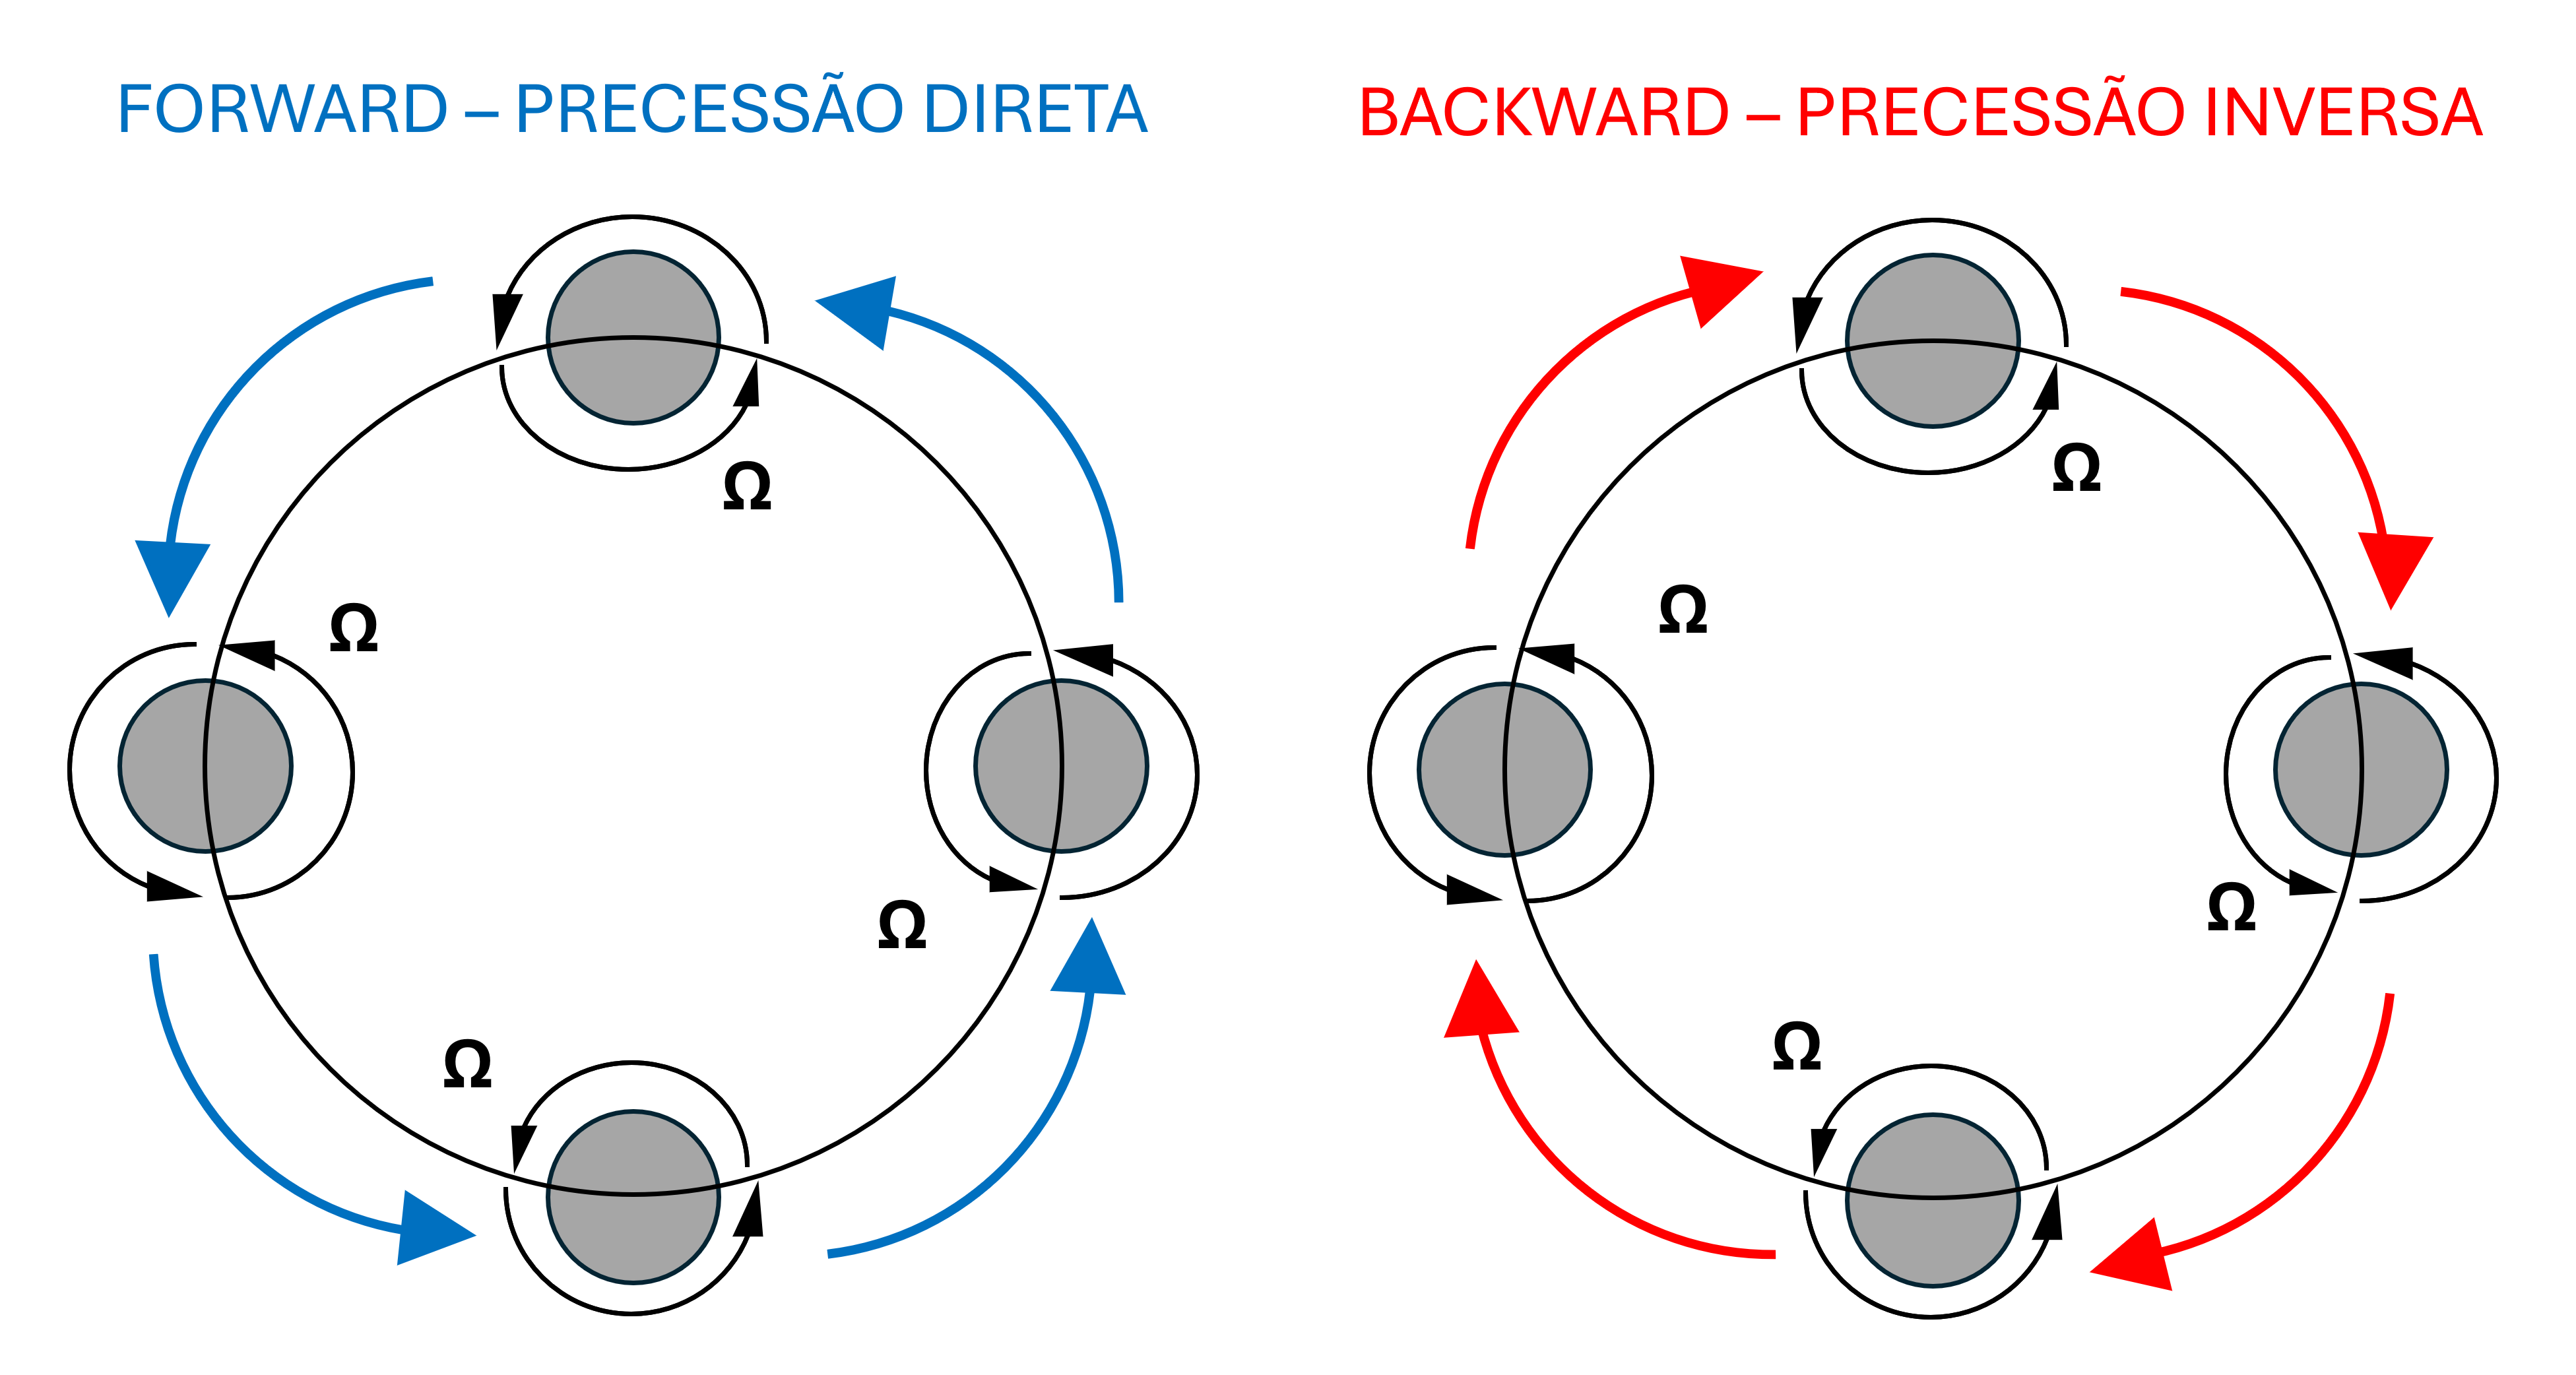
\includegraphics[width=\linewidth]{figuras/precessao.png}
		\par\vspace{0.3em}
		\raggedright
		{\small Fonte: Elaborado pelo autor.}
	\end{minipage}
\end{figure}

A Figura \ref{fig:campbell} apresenta o Diagrama de Campbell onde é possível visualizar que para cada velocidade de rotação $\Omega$ o sistema apresenta duas frequências naturais para cada modo lateral de vibração. Além disso,  ainda é possível é perceber que este exemplo apresenta o modo de vibrar torcional, ao qual não tem sua frequência natural alterada com a velocidade de rotação. A linha pontilhada faz a associação entre os valores de velocidade de rotação e frequência natural do rotor, conhecida como Linha de 1X e é essencial para a identificação das velocidades críticas, ou seja, indica qual velocidade coincide com uma frequência de vibração.
\begin{figure}[H]
	\centering
	\caption{Diagrama de Campbell}
	\label{fig:campbell}
	
	\begin{minipage}{0.7\textwidth}
		\centering
		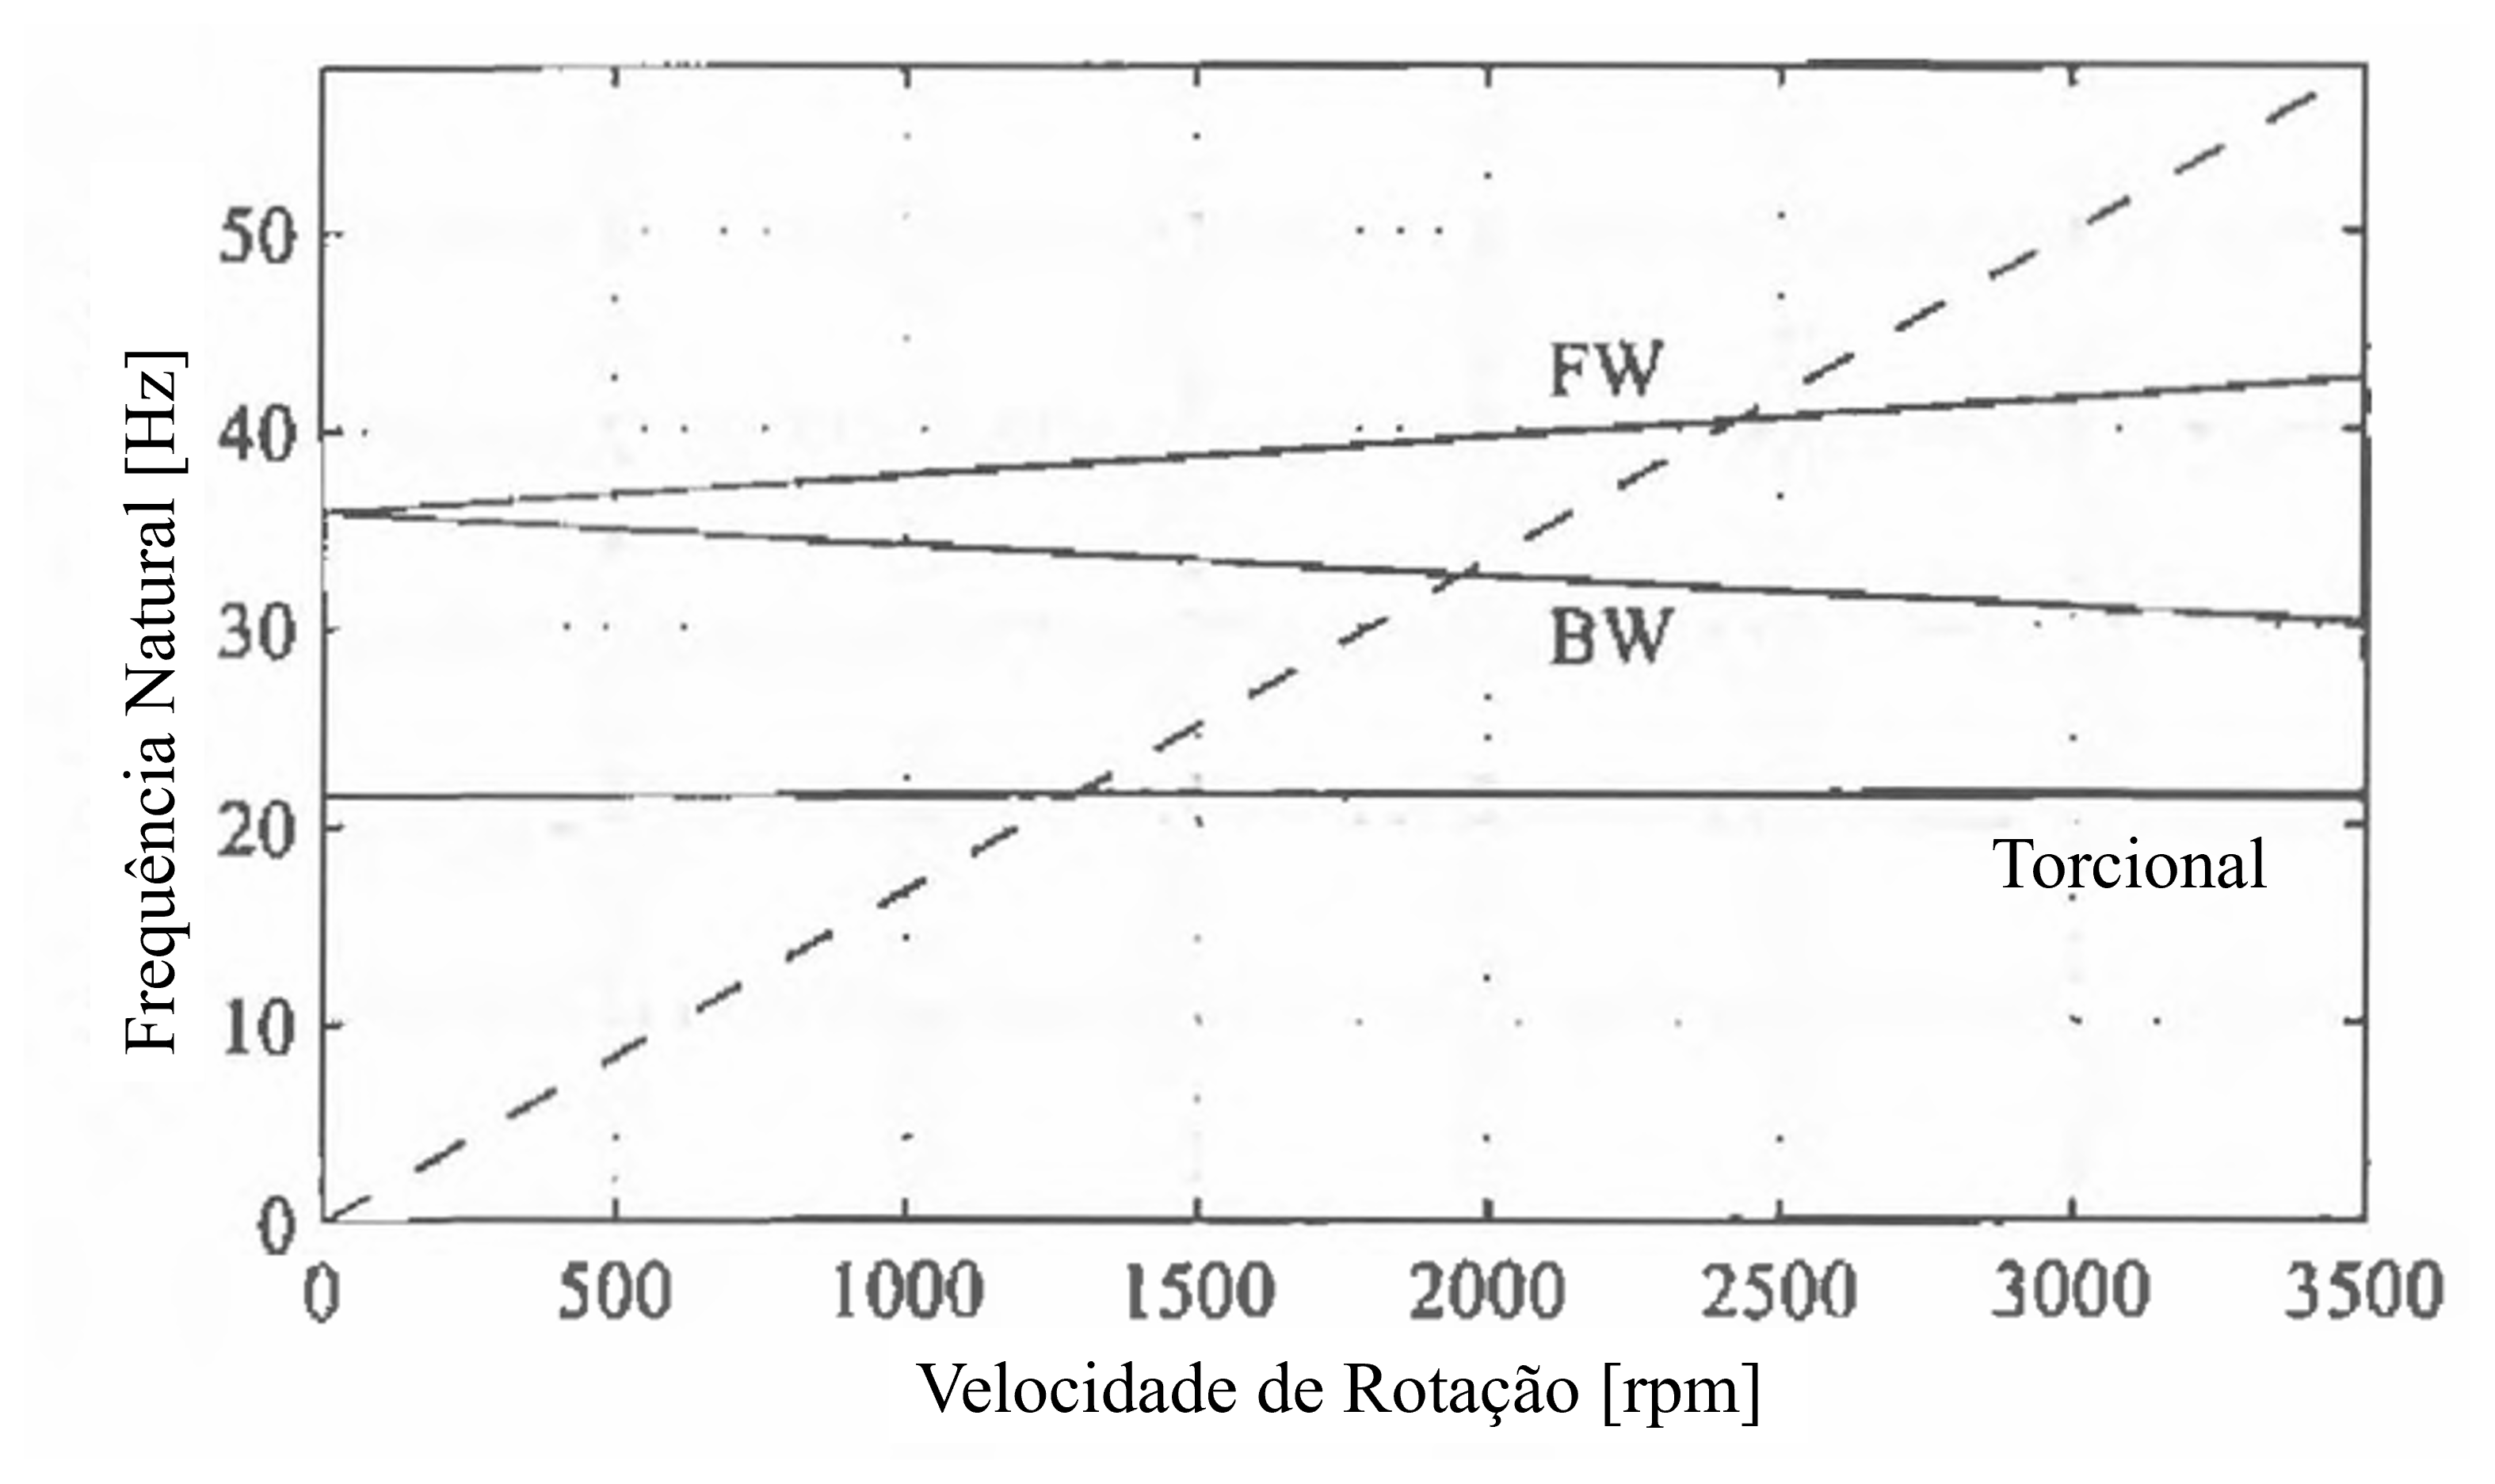
\includegraphics[width=\linewidth]{figuras/campbell.png}
		\par\vspace{0.3em}
		\raggedright
		{\small Fonte: Adaptado de \citeonline{Friswell2010}}
	\end{minipage}
\end{figure}

Dessa maneira, a correta modelagem matemática é essencial para o desenvolver análises e resultados robustos, coerentes e confiáveis. Assim, um modelo de elementos finitos para rotores foi desenvolvido por \citeonline{cavalini2013} com base na modelagem apresentada por \citeonline{Lalanne1998} servindo como referência para diversos trabalhos. Tal modelo contempla quatro graus de liberdade por nó, a expansão para seis \textit{gdl} pro nó foi apresentada por \citeonline{sicchieri2024}, assim como mostrado na Equação \ref{Eq:dof}.

O primeiro passo para a modelagem é definir a formulação da energia cinética e potencial para os elementos de eixo, discos, engrenagens, mancais e selos para posteriormente aplicar a metodologia de Lagrange e, enfim, obter as equações do movimentos. A Equação \ref{eq:lagrange_rot} apresenta o formalismo da equação de Lagrange para um vetor $q$ com $N$ graus de liberdade (Equação \ref{Eq:dof}). 
\begin{equation}
	\frac{\mathrm{d} }{\mathrm{d} t}\left ( \frac{\partial T}{\partial \dot{q_i}} \right )-\frac{\partial T}{\partial q_i} + \frac{\partial U}{\partial q_i}=F_{qi}
	\label{eq:lagrange_rot}
	\quad (i = 1, 2, ... N)
\end{equation}

Para este modelo, algumas considerações feitas são:
\begin{itemize}
	\item O eixo é representado como um elemento de viga com seção circular constante, de acordo com a Teoria de \citeonline{timoshenko1922}. É caracterizado por energia cinética e potencial, onde cada elemento possui dois nós e seis graus de liberdade por nó;
	\item O disco é um elemento rígido, logo possui apenas energia cinética;
	\item Engrenagens podem ser representadas como elementos de disco e estes são adicionados em nós;
	\item Os mancais e selos podem ser representados por um conjunto de molas e amortecedores lineares.
\end{itemize}

Assim, realizando o procedimento matemático necessário, obtêm-se a equação diferencial que representa o comportamento dinâmico de um rotor dada pela Equação \ref{Eq:movement}. Em que a velocidade de rotação é representada por $\Omega$.
\begin{equation}
	[M]\{\ddot{q}(t)\}+([C]+\Omega [G])\{\dot{q}(t)\}+[K]\{q(t)\}=\{F(t)\}
	\label{Eq:movement}
\end{equation}
\begin{equation}
	\{q\} = \{q_0, q_1, q_2, ..., q_N\}^{T}
	\quad (i = 1, 2, ... N)
	\label{Eq:dof}
\end{equation}

Onde $[M]$, $[C]$, $[G]$ e $[K]$ são as matrizes de massa, amortecimento, efeito giroscópico e rigidez, respectivamente, e $\{\ddot{q}(t)\}$, $\{\dot{q}(t)\}$, $\{q(t)\}$, e $\{F(t)\}$ são os vetores de aceleração, velocidade, deslocamento e força de entrada de todo o sistema, respectivamente, de acordo com os \textit{gdl} por nó dados pela Equação \ref{Eq:dof}.
\begin{equation}
	\{q_i\} = \{x_i,y_i,z_i, {\theta_x}_i, {\theta_y}_i, {\theta_z}_i\}^{T}
	\label{Eq:dof}
\end{equation}

Onde $x_i$, $y_i$ e $z_i$ correspondem às translações horizontal, vertical e axial, respectivamente. As variáveis ${\theta_x}_i$, ${\theta_y}_i$ e ${\theta_z}_i$ representam a flexão no plano $yz$, a flexão no plano $xz$ e a torção, respectivamente.

A \ref{subfigure:modelo} apresenta uma representação de um rotor real com mancais $B1$ e $B2$, disco $D1$ e velocidade $\Omega$ sua modelagem matemática com coeficientes de amortecimento ${C_b}_1$, ${C_b}_2$ e de rigidez ${K_b}_1$ e ${K_b}_2$.
\begin{figure}[H]
	\centering
	\caption{Subfiguras}
	\label{subfigure:modelo}
	
	\begin{minipage}{0.9\textwidth}
		\centering
		
		\begin{subfigure}{0.45\textwidth}
			\centering
			\caption{Esquema de rotor}
			\label{fig:rotor1}
			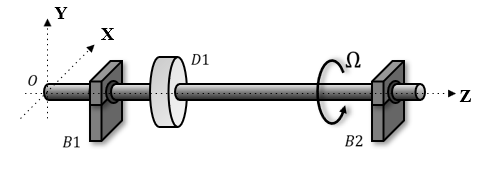
\includegraphics[width=\linewidth]{figuras/rotor1.png}
		\end{subfigure}
		\hspace{10pt}
		\begin{subfigure}{0.45\textwidth}
			\centering
			\caption{Representação do modelo}
			\label{fig:rotors}
			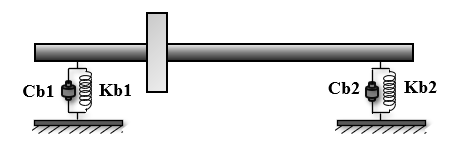
\includegraphics[width=\linewidth]{figuras/rotor2.png}
		\end{subfigure}
		
		\par\vspace{0.5em}
		\raggedright
		{\small Fonte: Elaborado pelo autor.}
	\end{minipage}
\end{figure}

Com a Equação do Movimento (Equação \ref{Eq:movement}) do sistema é possível determinar a resposta deste à forças aplicadas no vetor ${F(t)}$, determinar as frequências naturais, funções de resposta em frequência, resposta de desbalanceamento e diversas outras análises de dinâmica de rotação. 

%------------------------------------------------------------
%
%{\color{green} Nesta seção são apresentados os conceitos fundamentais utilizados no desenvolvimento desta dissertação de mestrado. Esses conceitos incluem: a modelagem matemática da rigidez de acoplamento de um par de engrenagens e o equacionamento de rotores flexíveis, empregado na simulação e validação da implementação de engrenamento.}
%
%\subsection{Modelo de rotores flexíveis}
%
%Um rotor flexível é um sistema dinâmico formado por discos, engrenagens, eixos flexíveis, mancais e selos. O modelo leva em consideração a geometria e as características de inércia, rigidez e amortecimento do sistema. Para obter a equação de movimento do rotor, os passos são: calcular a energia cinética e potencial dos componentes, escolher um método de discretização e aplicar as equações de Lagrange (Eq. \ref{eq_lalanne}) \cite{Lalanne1998}.
%\begin{equation}
%	\frac{\mathrm{d} }{\mathrm{d} t}\left ( \frac{\partial T}{\partial \dot{q_i}} \right )-\frac{\partial T}{\partial q_i} + \frac{\partial U}{\partial q_i}=F_{qi}
%	\label{eq_lalanne}
%	\quad (i = 1, 2, ... N)
%\end{equation}
%
%Onde $N$ é o número de graus de liberdade do sistema e o índice $i$ varia entre $1 \leq i \leq N$, $q_{i}$ são as coordenadas generalizadas, $F_{qi}$ são as forças generalizadas e $T$ e $U$ são as energias cinéticas e potenciais dos componentes, respectivamente.
%Para este modelo, algumas considerações feitas são:
%\begin{itemize}
%	\item O disco é um elemento rígido, logo possui apenas energia cinética;
%	\item Engrenagens podem ser representadas como elementos de disco e estes são adicionados em nós;
%	\item O eixo é representado como um elemento de viga com seção circular constante e é caracterizado por energia cinética e potencial, onde cada elemento possui dois nós e seis graus de liberdade por nó;
%	\item Os mancais e selos podem ser representados por um conjunto de molas e amortecedores lineares.
%\end{itemize}
%
%Assim, a equação diferencial que representa o comportamento dinâmico de um rotor é dada pela Eq. \ref{Eq:movement}.
%\begin{equation}
%	[M]\{\ddot{q}(t)\}+([C]+\Omega [G])\{\dot{q}(t)\}+[K]\{q(t)\}=\{F(t)\}
%	\label{Eq:movement}
%\end{equation}
%
%Onde $[M]$, $[C]$, $[G]$ e $[K]$ são as matrizes de massa, amortecimento, efeito giroscópico e rigidez, respectivamente, e $\{\ddot{q}(t)\}$, $\{\dot{q}(t)\}$, $\{q(t)\}$, e $\{F(t)\}$ são os vetores de aceleração, velocidade, deslocamento e força de entrada, respectivamente. A velocidade de rotação é representada por $\Omega$.
%
%O modelo ROSS, proposto por \citeonline{timbo2020}, utiliza a formulação de seis graus de liberdade para cada nó, três de translação e três de rotação, conforme mostrado abaixo e de acordo com \citeonline{Friswell2010}.
%\begin{equation}
%	\{q(t)\} = \{x,y,z, \theta_x, \theta_y, \theta_z\}^{T}
%	\label{Eq:dof}
%\end{equation}
%
%Onde $x$, $y$ e $z$ correspondem às translações horizontal, vertical e axial, respectivamente. As variáveis $\theta_x$, $\theta_y$ e $\theta_z$ representam a flexão no plano $yz$, a flexão no plano $xz$ e a torção, respectivamente.
%\begin{figure}[H]
%	\centering
%	\caption{Subfiguras}
%	\label{subfigure}
%	
%	\begin{minipage}{0.9\textwidth}
%		\centering
%		
%		\begin{subfigure}{0.45\textwidth}
%			\centering
%			\caption{Esquema de rotor}
%			\label{fig:rotor1}
%			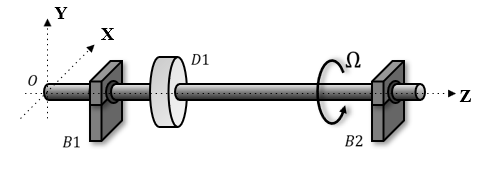
\includegraphics[width=\linewidth]{figuras/rotor1.png}
%		\end{subfigure}
%		\hspace{10pt}
%		\begin{subfigure}{0.45\textwidth}
%			\centering
%			\caption{Representação do modelo}
%			\label{fig:rotors}
%			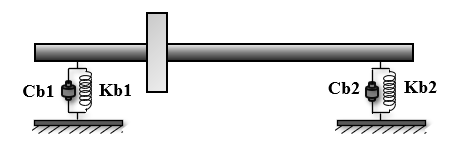
\includegraphics[width=\linewidth]{figuras/rotor2.png}
%		\end{subfigure}
%		
%		\par\vspace{0.5em}
%		\raggedright
%		{\small Fonte: Elaborado pelo autor.}
%	\end{minipage}
%\end{figure}
%
%
%\citeonline{jessica2025} Apresenta dados sobre a utilização mundial do pacote ROSS, juntamente com exemplos de utilização e resultados comparativos.
%
%--------------------------------------------------------------
%
%\section{Fundamentos da Dinâmica de Rotores - Gemini}
%
%A dinâmica de rotores dedica-se ao estudo do comportamento vibratório de estruturas mecânicas rotativas sujeitas a forças dinâmicas induzidas tanto pela rotação do próprio eixo quanto por interações externas, como o engrenamento de engrenagens. Diferente de estruturas estáticas, sistemas rotativos possuem equações de movimento cujas matrizes dependem diretamente da velocidade angular, introduzindo efeitos giroscópicos e forças não-conservativas que modificam a estabilidade e as frequências naturais do conjunto \cite{shigley2020}.
%
%A equação diferencial que governa o comportamento dinâmico linear de um sistema de rotores discretizado por Elementos Finitos (MEF) é expressa pela Eq.~\ref{eq:mov_rotores}:
%\begin{equation}
%	[M]\{\ddot{q}(t)\} + ([C] + \Omega [G])\{\dot{q}(t)\} + [K]\{q(t)\} = \{F(t)\}
%	\label{eq:mov_rotores}
%\end{equation}
%
%Em que $[M]$ representa a matriz de massa global, que computa a inércia translacional e rotacional do eixo e dos componentes acoplados (como discos e engrenagens). A matriz $[C]$ descreve o amortecimento viscoso estacionário proveniente dos mancais, vedações e amortecimento interno do material. O vetor $\{q(t)\}$ denota as coordenadas generalizadas de deslocamento nos nós do sistema, e $\{F(t)\}$ representa o vetor de forças externas aplicadas, tais como as forças de desbalanceamento e as forças induzidas pelo contato físico na malha de engrenamento.
%
%O termo $\Omega [G]$ introduz a \textbf{matriz giroscópica ($[G]$)} multiplicada pela velocidade de rotação do rotor ($\Omega$). Esse efeito atua de maneira antissimétrica acoplando os planos de vibração laterais ortogonais (por exemplo, os planos $x-z$ e $y-z$). Fisicamente, o efeito giroscópico gera o fenômeno de precessão (*whirl*), dividindo cada frequência natural do rotor em duas ramificações distintas: a precessão direta (*forward precession*), na qual o eixo orbita no mesmo sentido da rotação $\Omega$, e a precessão reversa (*backward precession*), onde a órbita ocorre no sentido oposto.
%
%A \textbf{matriz de rigidez global ($[K]$)} agrega a rigidez flexional estrutural do eixo e os coeficientes de rigidez diretos e cruzados dos elementos de suporte, como os mancais hidrodinâmicos ou de rolamento. Em sistemas acoplados por engrenagens, a rigidez total do sistema sofre a inclusão da matriz de acoplamento $[K_{mesh}]$, conforme visto na Eq.~\ref{Eq:mov-alt}, estruturando um vínculo dinâmico altamente não-linear e dependente da posição instantânea das engrenagens.
%
%\subsection{Principais Análises e Atividades em Dinâmica de Rotores}
%
%Para garantir a integridade estrutural e operacional de uma turbomáquina ou redutor industrial, diferentes análises numéricas devem ser executadas a partir da Eq.~\ref{eq:mov_rotores}. As atividades fundamentais dividem-se em:
%
%\begin{itemize}
%	\item \textbf{Análise de Autovalores e Diagrama de Campbell:} Soluciona-se a equação homogênea livre de forças para determinar as frequências naturais amortecidas ($\omega_d$) em função da variação da velocidade de rotação $\Omega$. O cruzamento dessas frequências com as linhas de excitação síncronas ($1\times\Omega$, originada por desbalanceamento) ou sub/supersíncronas (como a frequência de engrenamento $Z_1\Omega$) estabelece as \textbf{velocidades críticas} do rotor. O Diagrama de Campbell é a ferramenta gráfica utilizada para mapear essas interseções e projetar margens de segurança operacionais.
%	\item \textbf{Análise de Estabilidade Flutante:} A partir dos autovalores complexos $\lambda_i = \sigma_i \pm i\omega_{di}$, avalia-se o amortecimento do sistema através do \textbf{decremento logarítmico ($\delta_{log}$)}, definido pela Eq.~\ref{eq:dec_log}:
%	\begin{equation}
%		\delta_{log} = -\frac{2\pi \sigma_i}{\omega_{di}}
%		\label{eq:dec_log}
%	\end{equation}
%	Se a parte real $\sigma_i$ tornar-se positiva ($\delta_{log} < 0$), o sistema assume um comportamento instável, caracterizado por vibrações autoexcitadas divergentes, associadas frequentemente a efeitos de perseguição de óleo (*oil whirl/whip*) em mancais hidrodinâmicos ou forças cruzadas de engrenamento.
%	\item \textbf{Resposta ao Desbalanceamento Síncrono:} Avalia-se o comportamento em regime permanente do rotor sob a ação de forças centrífugas geradas por excentricidades de massa residuais, como as descritas nas Eqs.~\ref{eq:desbal_eng1} e \ref{eq:desbal_eng2}. Essa análise quantifica a amplitude de vibração nos nós críticos e a força transmitida aos mancais, validando os critérios de projeto de acordo com normas vigentes.
%	\item \textbf{Análise de Órbitas e Resposta Transiente no Tempo:} Consiste na integração numérica direta das equações de movimento quando submetidas a excitações não-lineares severas, como a transição do contato no dente devido ao \textit{backlash} ou efeitos de impacto. A plotagem do deslocamento horizontal contra o vertical ($x_i \times y_i$) desenha a órbita dinâmica do nó, permitindo identificar regimes de sub-harmônicos, caos ou perda de contato na transmissão.
%\end{itemize}
%
%---
